\chapter{SHA-3 finalists : Gr$\o$stl, BLAKE, and Keccak}

\section{Gr$\o$stl}

Gr$\o$stl is collection of hash functions which produce digest size, ranging from 1 to 64 bytes. The variant of
Gr$\o$stl that returns a message digest of size n, is called Gr$\o$stl-n.

Gr$\o$stl is an iterated hash function, with two two compression functions named P and Q, based on wide trail design
and having distinct permutations. Gr$\o$stl has a byte oriented SP network, and its diffusion layers and S-box 
are identical to AES. The design is a wide-pipe construction, where the internal state size is larger than output 
size. Thus preventing most of the generic attacks. None of the permutations are indexed by a key, to prevent attacks
from a weak key schedule. \cite{00019}

  \subsection{The hash function construction}

  The input is padded and then split into l-bit message blocks $m_{1}$,$\ldots$, $m_{t}$, and each message block is
  processed sequentially. The initial l-bit chaining value $h_{0}$ = iv is defined, and the blocks $m_{i}$ are
  processed as 

  $ h_{i}\gets f(h_{i-1}, m_{i})$ for i = 1,$\ldots$, t. 

  Thus f consumes two $l-bits$ input, and maps to output of $l-bits$. For variants up to 256 bits output, size of $l$ is
  256 bits. And for digest sizes larger than 256 bits, $l$ is 1024 bits.

  \begin{figure}
    \begin{center}
      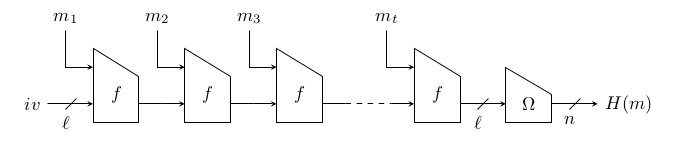
\includegraphics[width=5.5in]{groestlhashfunction.jpg}
    \end{center}
    \caption{Gr$\o$stl hash function}
    \label{fig:lab}
  \end{figure}

  After the last message block is processed, the last chaining value output is sent through a $\Omega$ function, to get
  the hash output H(M).

  $H(M) = \Omega(h_{t}),$

  The entire process is shown in the above figure 3.1.

  The f function shown above, is composed of two l-bit permutations called P and Q, which is defined as follows.

  $f(h, m) = P(h \oplus m) \oplus Q(m) \oplus h.$
  
  \begin{figure}[h]
    \begin{center}
      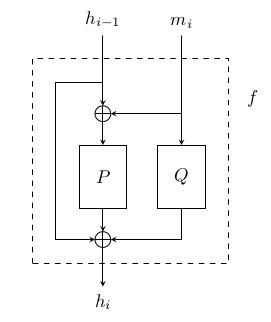
\includegraphics[width=2.5in]{groestlPQfunction.jpg}
    \end{center}
    \caption{Compression functions, where P and Q are $l-bit$ permutations}
    \label{fig:lab}
  \end{figure}

  The $\Omega$ function consists of a $trunc_{n}(x)$ that outputs only the trailing n bits of input x. The $\Omega$ function
  can now be defined as 

  $\Omega(x) = trunc_{n}( P(x) \oplus x ).$

  \begin{figure}[h]
    \begin{center}
      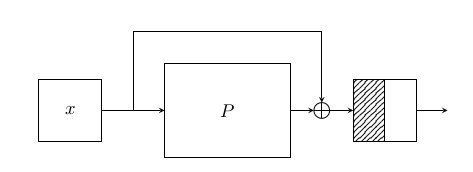
\includegraphics[width=4.5in]{groestlomegafunction.jpg}
    \end{center}
    \caption{Omega truncation function}
    \label{fig:lab}
  \end{figure}

  In order to fit the varying input length message to the block sizes of $ l $ padding is defined. First bit '1' is
  appended, then $ w = -N - 65 mod l $ 0 bits are appended; where N is the length of the original message. Finally a
  64 bit representation of $(N + w + 65) / l $. Given the need for message length, the maximum size of message digest
  in bits for Gr$\o$stl-512 version is $2^{73}-577$ bits, and that for 1024 version is $2^{74}-1089$bits.

  \subsection{Design of P and Q permutations}

  There are two variations for P and Q permutations, one each for the digest size lower and higher than 256 bits. There
  are four round transformations, that compose a round R. The permutation consists of a number of rounds R. R can be
  represented as 

  $ R = MixBytes \cdot ShiftBytes \cdot SubBytes \cdot AddRoundConstant $

  The transformations SubBytes and MixBytes are same for all transformation while, ShiftBytes and AddRoundConstant differ
  for each of the transformations. The transformations operate on matrix of bytes, with the permutation of lower size
  digest having matrix of 8 rows and 8 columns, while that for larger variant is of 16 columns and 8 rows. The mapping of
  the input to the state and the transformations are explained below. The number of rounds for each R is given as 
  recommendation in table 3.1 and the initial values are given in table 3.2
  
  \begin{table}
    \begin{center}
      \begin{tabular}{ *{3}{c} } \hline
        Permutations            & Digest size & Recommended value of r \\ \hline
        $P_{512}$ and $Q_{512}$   & 8 - 256     & 10 \\
        $P_{1024}$ and $Q_{1024}$ & 264 - 512   & 14 \\ \hline 
      \end{tabular}
      \caption{Recommended number of rounds}
    \end{center}
  \end{table}

  \begin{table}
    \begin{center}
      \begin{tabular}{ *{2}{c} } \hline
        n   & $iv_{n}$         \\ \hline
        224 & 00 $\dots$ 00 00 e0 \\
        256 & 00 $\dots$ 00 01 00 \\
        384 & 00 $\dots$ 00 01 80 \\
        512 & 00 $\dots$ 00 02 00 \\ \hline
      \end{tabular}
    \caption{Above are initial values for Gr$\o$stl-n function. The numbers on left denote digest size in bits.}
    \end{center}
  \end{table}


  \begin{itemize}
    \item {\bf Mapping:} of a 64-byte sequence of 00 01 02 $\ldots$ 3f to a 8 $\times$ 8 matrix is shown in the following matrix.
    For a 8 $\times$ 16 matrix, the mapping is extended the same way. Mapping the intermediate state values to byte sequence
    would be reverse of this.
      $ Input Mapping = \begin{bmatrix}
        00 & 08 & 10 & 18 & 20 & 28 & 30 & 38 \\
        01 & 09 & 11 & 19 & 21 & 29 & 31 & 39 \\
        02 & 0a & 12 & 1a & 22 & 2a & 32 & 3a \\
        03 & 0b & 13 & 1b & 23 & 2b & 33 & 3b \\
        04 & 0c & 14 & 1c & 24 & 2c & 34 & 3c \\
        05 & 0d & 15 & 1d & 25 & 2d & 35 & 3d \\
        06 & 0e & 16 & 1e & 26 & 2e & 36 & 3e \\
        07 & 0f & 17 & 1f & 27 & 2f & 37 & 3f
      \end{bmatrix}$
    \item {\bf AddRoundConstant:} transformation round XOR a round dependant constant to the state matrix say A. It is
    represented as $A \gets A \oplus C[i]$, where C[i] is the round constant in round i. The constants for both P and Q for both
    variations are given below.

    $ P_{512}: C[i] = \begin{bmatrix}
      00 \oplus i & 10 \oplus i & 20 \oplus i & 30 \oplus i & 40 \oplus i & 50 \oplus i & 60 \oplus i & 70 \oplus i \\
      00     & 00     & 00     & 00     & 00     & 00     & 00     & 00     \\
      00     & 00     & 00     & 00     & 00     & 00     & 00     & 00     \\
      00     & 00     & 00     & 00     & 00     & 00     & 00     & 00     \\
      00     & 00     & 00     & 00     & 00     & 00     & 00     & 00     \\
      00     & 00     & 00     & 00     & 00     & 00     & 00     & 00     \\
      00     & 00     & 00     & 00     & 00     & 00     & 00     & 00     \\
      00     & 00     & 00     & 00     & 00     & 00     & 00     & 00     \\
    \end{bmatrix}$

    and 

    $Q_{512}: C[i] = \begin{bmatrix}
      ff     & ff     & ff     & ff     & ff     & ff     & ff     & ff     \\
      ff     & ff     & ff     & ff     & ff     & ff     & ff     & ff     \\
      ff     & ff     & ff     & ff     & ff     & ff     & ff     & ff     \\
      ff     & ff     & ff     & ff     & ff     & ff     & ff     & ff     \\
      ff     & ff     & ff     & ff     & ff     & ff     & ff     & ff     \\
      ff     & ff     & ff     & ff     & ff     & ff     & ff     & ff     \\
      ff     & ff     & ff     & ff     & ff     & ff     & ff     & ff     \\
      ff \oplus i & ef \oplus i & df \oplus i & cf \oplus i & bf \oplus i & af \oplus i & 9f \oplus i & 8f \oplus i 
    \end{bmatrix}$

    Similarly, the P and Q for the wider variants are written.

    $ P_{1024}: C[i] = \begin{bmatrix}
      00 \oplus i & 10 \oplus i & 20 \oplus i & 30 \oplus i & 40 \oplus i & 50 \oplus i & 60 \oplus i & 70 \oplus i \ldots f0 \oplus i \\
      00     & 00     & 00     & 00     & 00     & 00     & 00     & 00     \dots 00 \\
      00     & 00     & 00     & 00     & 00     & 00     & 00     & 00     \dots 00 \\
      00     & 00     & 00     & 00     & 00     & 00     & 00     & 00     \dots 00 \\
      00     & 00     & 00     & 00     & 00     & 00     & 00     & 00     \dots 00 \\
      00     & 00     & 00     & 00     & 00     & 00     & 00     & 00     \dots 00 \\
      00     & 00     & 00     & 00     & 00     & 00     & 00     & 00     \dots 00 \\
      00     & 00     & 00     & 00     & 00     & 00     & 00     & 00     \dots 00 \\
    \end{bmatrix}$

    and 

    $Q_{512}: C[i] = \begin{bmatrix}
      ff     & ff     & ff     & ff     & ff     & ff     & ff     & ff     \dots ff    \\
      ff     & ff     & ff     & ff     & ff     & ff     & ff     & ff     \dots ff    \\
      ff     & ff     & ff     & ff     & ff     & ff     & ff     & ff     \dots ff    \\
      ff     & ff     & ff     & ff     & ff     & ff     & ff     & ff     \dots ff    \\
      ff     & ff     & ff     & ff     & ff     & ff     & ff     & ff     \dots ff    \\
      ff     & ff     & ff     & ff     & ff     & ff     & ff     & ff     \dots ff    \\
      ff     & ff     & ff     & ff     & ff     & ff     & ff     & ff     \dots ff    \\
      ff \oplus i & ef \oplus i & df \oplus i & cf \oplus i & bf \oplus i & af \oplus i & 9f \oplus i & 8f \oplus i \dots 0f \oplus i
    \end{bmatrix}$

    where i is the round number represented as 8 bits value, and all other numbers are represented as
    hexadecimals.

  \item {\bf SubBytes:} substitutes each byte in state by value from S-box. The S-box is described in appendix
  A. Say $a_{i,j}$ a element in row i and column j of the state matrix, then the transformation done is 
  $a_{i,j} \gets S( a_{i,j}),  0 \leq i < 8, 0 \leq j < v.$ 
  
  \begin{figure}[h]
    \begin{center}
      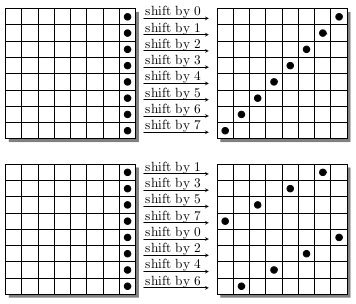
\includegraphics[width=3.6in]{groestl512shift.jpg}
    \end{center}
    \caption{ShiftBytes transformation of permutation $P_{512}$(top) and $Q_{512}$(bottom)}
    \label{fig:lab}
  \end{figure}

  \newpage

  \item {\bf ShiftBytes:} transformation cyclically shifts the bytes in a row to left by that number. Let list 
  vector of a number denote the shift, with the index of the element indicating the row. The vector representation
  for $P_{512}$ = [0, 1, 2, 3, 4, 5, 6, 7] and $Q_{512}$ = [1, 3, 5, 7, 0, 2, 4, 6]. The shift is shown in figure
  3.4. Those for the larger permutation are $P_{1024}$ = [0, 1, 2, 3, 4, 5, 6, 11]and $Q_{1024}$ = 
  [1, 3, 5, 11, 0, 2, 4, 6]. This shifting is shown in figure 3.5.
    
  \begin{figure}
    \begin{center}
      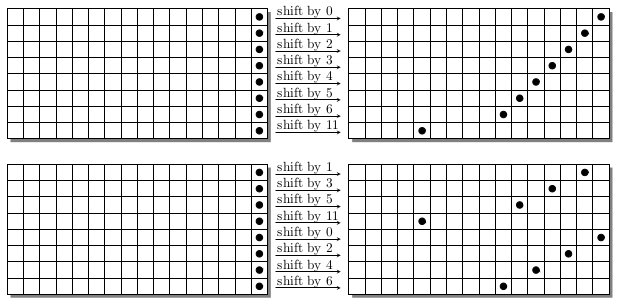
\includegraphics[width=6.4in]{groestl1024shift.jpg}
    \end{center}
    \caption{ShiftBytes transformation of permutation $P_{1024}$(top) and $Q_{1024}$(bottom)}
    \label{fig:lab}
  \end{figure}

  \item {\bf MixBytes:} transformation, multiplies each column of the state matrix A, by a constant 8 $\times$ 8 matrix B.
  The transformation, can be shown as $ A \gets B \times A$. The matrix B, can be seen as a finite field over $\mathbb{F}_{256}$.
  This finite field is defined over $\mathbb{F}_{2}$ by the irreducible polynomial $x^{8} \oplus x^{4} \oplus x^{3} \oplus x \oplus 1$.
  The composition of matrix B is shown, in appendix A, in item 2.
  %The bytes of the state matrix are in $\mathbb{F}_{256}$ in polynomials of degree at most 7, and coefficients in 0 and 1.
  %The matrix B, is circular shifting of the same row. Each row of the matrix below the current row, is rotated left by
  %a place.

  \end{itemize}

\section{BLAKE} 

BLAKE\cite{00002} hash function is built on HAIFA (HAsh Iterative FrAmework) structure \cite{00020} which is an improved
version of Merkle-Damg$\dot{a}$rd function. And provides resistance to long-message second pre-image attack as well as
provides a salting option, that BLAKE uses\cite{00021}.
The design is local wide-pipe which avoids internal collisions. The compression function in BLAKE is tweaked version of 
ChaCha, a stream cipher. 

\begin{table}[h]
  \begin{center}
    \begin{tabular}{ *{6}{c} } \hline
      Algorithm & Word & Message    & Block & Digest & Salt \\ \hline
      BLAKE-224 & 32   & $< 2^{64}$  & 512   & 224    & 128  \\
      BLAKE-256 & 32   & $< 2^{64}$  & 512   & 256    & 128  \\
      BLAKE-384 & 64   & $< 2^{128}$ & 1024  & 384    & 256  \\
      BLAKE-512 & 64   & $< 2^{128}$ & 1024  & 512    & 256  \\ \hline
    \end{tabular}
    \caption{Specification of available input, output, block and salt sizes for various BLAKE hash functions.}
  \end{center}
\end{table}

\begin{figure}[h]
  \begin{center}
    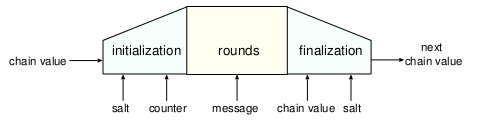
\includegraphics[width=4.75in]{blakelocalwidepipeconstruction.jpg}
  \end{center}
  \caption{Local wide construction of BLAKE's compression function}
  \label{fig:lab}
\end{figure}

As seen from table 3.3, BLAKE has 4 variations of the algorithm that can give only 4 different digest lengths. The input
length is also smaller than Gr$\o$stl. Figure 3.6 shows how the individual message blocks are consumed. The construction
takes in 4 inputs, one message; two a salt, that makes function that parameter specific; and three a counter, which is 
count of all the bits hashed till then; and lastly a chaining value which is input of the previous operation or initial
value in case of hash initiation. The compression function is composed of a 4 $\times$ 4 matrix of words. Where one word is 
equal to 32 bits for BLAKE-256 variant, while 64 bit for variant BLAKE-512.

\begin{table}[h]
  \begin{center}
    \begin{tabular}{ c l } \hline
      Symbol                 & Meaning \\ \hline
      $\gets$                    & variable assignment \\
      $+$                    & addition modulo $2^{32}$ or (modulo $2^{64}$) \\
      $\gg k$                  & rotate k bits to least significant bits \\
      $\ll k$                  & rotate k bits to most significant bits \\
      $\langle l \rangle_{k}$ & encoding of integer $l$ over $k$ bits \\ \hline
    \end{tabular}
    \caption{Convention of symbols used in BLAKE algorithm}
  \end{center}
\end{table}

\subsection{ BLAKE-256 }

The compression function takes following as input
\begin{itemize}
  \item a chaining value of $h = h_{0},\dots, h_{7}$
  \item a message block $m = m_{0},\dots, m_{15}$
  \item a salt $s = s_{0},\dots, s_{3}$
  \item a counter $t = t_{0}, t_{1}$
\end{itemize}
These four inputs of 30 words or 120 bytes, are processed as $h' = compress(h, m, s, t)$ to provide a new
chain value of 8 words.

  \subsubsection{Compression function}

  \begin{itemize}
    \item {\bf Constants}
      \begin{table}[h]
        \begin{center}
          \begin{tabular}{ *{4}{c}}
            $IV_{0}$ = 6A09E667 & $IV_{1}$ = BB67AE85 & $IV_{2}$ = 3C6EF372 & $IV_{3}$ = A54FF53A \\
            $IV_{4}$ = 510E527F & $IV_{5}$ = 9B05688C & $IV_{6}$ = 1F83D9AB & $IV_{7}$ = 5BE0CD19 \\
          \end{tabular}
          \caption{Initial values which become the chaining value for the first message block}
        \end{center}
      \end{table}
      
      \begin{table}[h]
        \begin{center}
          \begin{tabular}{ *{4}{c}}
            $c_{0}$  = 243F6A88 & $c_{1}$  = 85A308D3 & $c_{2}$  = 13198A2E & $c_{3}$  = 03707344 \\
            $c_{4}$  = A4093822 & $c_{5}$  = 299F31D0 & $c_{6}$  = 082EFA98 & $c_{7}$  = EC4E6C89 \\
            $c_{8}$  = 452821E6 & $c_{9}$  = 38D01377 & $c_{10}$ = BE5466CF & $c_{11}$ = 34E90C6C \\
            $c_{12}$ = C0AC29B7 & $c_{13}$ = C97C50DD & $c_{14}$ = B5470917 & $c_{15}$ = 3F84D5B5 \\
          \end{tabular}
          \caption{16 constants used for BLAKE-256}
        \end{center}
      \end{table}

      \begin{table}
        \begin{center}
          \begin{tabular}{ c| *{16}{c}} \hline
            $\sigma_{0}$ & 0  & 1  & 2  & 3  & 4  & 5  & 6  & 7  & 8  & 9  & 10 & 11 & 12 & 13 & 14 & 15 \\
            $\sigma_{1}$ & 14 & 10 & 4  & 8  & 9  & 15 & 13 & 6  & 1  & 12 & 0  & 2  & 11 & 7  & 5  & 3  \\
            $\sigma_{2}$ & 11 & 8  & 12 & 0  & 5  & 2  & 15 & 13 & 10 & 14 & 3  & 6  & 7  & 1  & 9  & 4  \\
            $\sigma_{3}$ & 7  & 9  & 3  & 1  & 13 & 12 & 11 & 14 & 2  & 6  & 5  & 10 & 4  & 0  & 15 & 8  \\
            $\sigma_{4}$ & 9  & 0  & 5  & 7  & 2  & 4  & 10 & 15 & 14 & 1  & 11 & 12 & 6  & 8  & 3  & 13 \\
            $\sigma_{5}$ & 2  & 12 & 6  & 10 & 0  & 11 & 8  & 3  & 4  & 13 & 7  & 5  & 15 & 14 & 1  & 9  \\
            $\sigma_{6}$ & 12 & 5  & 1  & 15 & 14 & 13 & 4  & 10 & 0  & 7  & 6  & 3  & 9  & 2  & 8  & 11 \\
            $\sigma_{7}$ & 13 & 11 & 7  & 14 & 12 & 1  & 3  & 9  & 5  & 0  & 15 & 4  & 8  & 6  & 2  & 10 \\
            $\sigma_{8}$ & 6  & 15 & 14 & 9  & 11 & 3  & 0  & 8  & 12 & 2  & 13 & 7  & 1  & 4  & 10 & 5  \\
            $\sigma_{9}$ & 10 & 2  & 8  & 4  & 7  & 6  & 1  & 5  & 15 & 11 & 9  & 14 & 3  & 12 & 13 & 0  \\ \hline
          \end{tabular}
          \caption{Round permutations to be used}
        \end{center}
      \end{table}
    
    \item {\bf Initialization: } The constants mentioned are used with the salts, and counter along with initial
    value used as chaining input, to create a initial matrix of 4 $\times$ 4, 16 word state.

    $\begin{pmatrix} v_{0} & v_{1} & v_{2} & v_{3} \\ v_{4} & v_{5} & v_{6} & v_{7} \\
                     v_{8} & v_{9} & v_{10} & v_{11} \\ v_{12} & v_{13} & v_{14} & v_{15}\end{pmatrix} 
    \gets
    \begin{pmatrix} h_{0} & h_{1} & h_{2} & h_{3} \\ h_{4} & h_{5} & h_{6} & h_{7} \\
       s_{0} \oplus c_{0} & s_{1} \oplus c_{1} & s_{2} \oplus c_{2} & s_{3} \oplus c_{3} \\ 
       t_{0} \oplus c_{4} & t_{0} \oplus c_{5} & t_{1} \oplus c_{6} & t_{1} \oplus c_{7} \end{pmatrix}$

    \item {\bf Round function:} After initialisation, the state is subjected to column and diagonal operations, 14
    times. A round operation G acts as per following

    \begin{table}
      \begin{center}
        \begin{tabular}{ *{4}{c}}
        $ G_{0}(v_{0}, v_{8}, v_{12})$ & $G_{1}(v_{1}, v_{5}, v_{9}, v_{13})$ & $G_{2}(v_{2}, v_{6}, v_{10}, v_{14})$ & $G_{3}(v_{3}, v_{7}, v_{11}, v_{15}) $\\
 $G_{4}(v_{0}, v_{5}, v_{10}, v_{15})$ & $G_{5}(v_{1}, v_{6}, v_{11}, v_{12})$ & $G_{6}(v_{2}, v_{7}, v_{8}, v_{13})$ & $G_{7}(v_{3}, v_{4}, v_{9}, v_{14})$
        \end{tabular}
      \end{center}
    \end{table}

    %$ G_{0}(v_{0}, v_{8}, v_{12}) \; G_{1}(v_{1}, v_{5}, v_{9}, v_{13}) \; G_{2}(v_{2}, v_{6}, v_{10}, v_{14}) \; G_{3}(v_{3}, v_{7}, v_{11}, v_{15}) \\
    %G_{4}(v_{0}, v_{5}, v_{10}, v_{15}) \; G_{5}(v_{1}, v_{6}, v_{11}, v_{12}) \; G_{6}(v_{2}, v_{7}, v_{8}, v_{13}) \; G_{7}(v_{3}, v_{4}, v_{9}, v_{14})$

    where the round function $G_{i}(a, b, c, d)$ sets
    
    $
    a \gets a + b + (m_{\sigma_{r}(21)} \oplus c_{\sigma_{r}(2i + 1)}) \\
    d \gets (d \oplus a) \gg 16 \\
    c \gets c + d \\
    b \gets (b \oplus c) \gg 12 \\
    a \gets a + b + (m_{\sigma_{r}(2i + 1)} \oplus c_{\sigma_{r}(2i)}) \\
    d \gets (d \oplus a) \gg 8 \\
    c \gets c + d \\
    b \gets (b \oplus c) \gg 7
    $

    The implementation of the G function is shown below.
    \begin{figure}[h]
      \begin{center}
        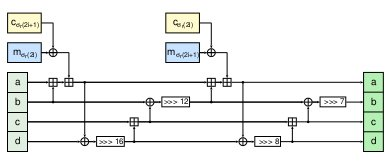
\includegraphics[width=4in]{blakeGfunction.jpg}
      \end{center}
      \caption{The $G_{i}$ function in BLAKE}
      \label{fig:lab}
    \end{figure}

    \item {\bf Finalization:} The chaining values for the next stage are obtained by XOR of the words from the state 
    matrix, the salt and the initial value.

    $
    h'_{0} \gets h_{0} \oplus s_{0} \oplus v_{0} \oplus v_{8} \\
    h'_{1} \gets h_{1} \oplus s_{1} \oplus v_{1} \oplus v_{9} \\
    h'_{2} \gets h_{2} \oplus s_{2} \oplus v_{2} \oplus v_{10} \\
    h'_{3} \gets h_{3} \oplus s_{3} \oplus v_{3} \oplus v_{11} \\
    h'_{4} \gets h_{4} \oplus s_{0} \oplus v_{4} \oplus v_{12} \\
    h'_{5} \gets h_{5} \oplus s_{1} \oplus v_{5} \oplus v_{13} \\
    h'_{6} \gets h_{6} \oplus s_{2} \oplus v_{6} \oplus v_{14} \\
    h'_{7} \gets h_{7} \oplus s_{3} \oplus v_{7} \oplus v_{15} \\
    $
  \end{itemize}

  \subsubsection{Hashing the message}

  A given input message is padded with a bit '1' followed followed by at most 511 bits of zeros, so that the message 
  size is equal to 447 modulo 512. This padding is followed by a bit '1' and a 64-bit unsigned big-endian representation
  of block length $l$. The padding to a message, can be represented as $m \gets m \parallel 1000 \dots 0001\langle l \rangle_{64}$

  \begin{algorithm}
  \caption{BLAKE Compression procedure}
  \begin{algorithmic}[1]
    \State $ h^{0} \gets IV $
    \For {$i = 0,\dots, N - 1$}
      \State $h^{i+1} \gets compress(h^{i}, m^{i}, s, l^{i})$
    \EndFor
    \State\Return{$h^{N}$}
  \end{algorithmic}
  \end{algorithm}

  As shown in algorithm 3.1, the BLAKE compression function ingests the padded message block by block, in a loop 
  starting from the initial value, and then sends the last chained value obtained from the finalization to the 
  $\Omega$ truncation function, to obtain the hash value.

\subsection{BLAKE-512}

operates on 64-bit words and returns a 64-byte hash value. The chaining value is 512 bit long, message blocks are
1024 bits, salt is 256 bits, and counter size is 128 bits. The difference from BLAKE-256 are in constants(tables 3.8 
and 3.9), compression function and the way message is padded.

  \begin{table}
    \begin{center}
      \begin{tabular}{ *{3}{c}}
        $IV_{0}$ = 6A09E667F3BCC908 & $IV_{1}$ = BB67AE8584CAA73B & $IV_{2}$ = 3C6EF372FE94F82B \\
        $IV_{3}$ = A54FF53A5F1D36F1 & $IV_{4}$ = 510E527FADE682D1 & $IV_{5}$ = 9B05688C2B3E6C1F \\
        $IV_{6}$ = 1F83D9ABFB41BD6B & $IV_{7}$ = 5BE0CD19137E2179 &                             \\
      \end{tabular}
      \caption{Initial values used for BLAKE-512}
    \end{center}
  \end{table}
  
  \begin{table}
    \begin{center}
      \begin{tabular}{ *{3}{c}}
        $c_{0}$  = 243F6A8885A308D3 & $c_{1}$  = 13198A2E03707344 & $c_{2}$  = A4093822299F31D0 \\
        $c_{3}$  = 082EFA98EC4E6C89 & $c_{4}$  = 452821E638D01377 & $c_{5}$  = BE5466CF34E90C6C \\
        $c_{6}$  = C0AC29B7C97C50DD & $c_{7}$  = 3F84D5B5B5470917 & $c_{8}$  = 9216D5D98979FB1B \\
        $c_{9}$  = D1310BA698DFB5AC & $c_{10}$ = 2FFD72DBD01ADFB7 & $c_{11}$ = B8E1AFED6A267E96 \\
        $c_{12}$ = BA7C9045F12C7F99 & $c_{13}$ = 24A19947B3916CF7 & $c_{14}$ = 0801F2E2858EFC16 \\
        $c_{15}$ = 636920D871574E69 &                             &                             \\
      \end{tabular}
      \caption{16 constants used for BLAKE-512}
    \end{center}
  \end{table}
  
  Compression function in BLAKE-512 gets 16 iterations instead of 14 as in BLAKE-256, as well the rotations
  are updated and word size increased from 32 bits to 64 bits. The $G_{i}(a, b, c, d)$ 
  is given as
  $
  a \gets a + b + (m_{\sigma_{r}(21)} \oplus c_{\sigma_{r}(2i + 1)}) \\
  d \gets (d \oplus a) \gg 32 \\
  c \gets c + d \\
  b \gets (b \oplus c) \gg 25 \\
  a \gets a + b + (m_{\sigma_{r}(2i + 1)} \oplus c_{\sigma_{r}(2i)}) \\
  d \gets (d \oplus a) \gg 16 \\
  c \gets c + d \\
  b \gets (b \oplus c) \gg 11
  $
  
  Once more than 9 rounds are done, the permutation table rules kick in, for example if round r \textgreater 9 then
  permutation used is $\sigma_{r \thickspace mod \thickspace 10}$, say r = 15 then permutation would be 
  $\sigma_{15 \thickspace mod \thickspace 10} = \sigma_{5}$.

  For the padding, the message is first padded with bit 1 and then as many zeros required to make the bit length
  equivalent to 895 modulo 1024. After that another bit of value 1 is appended followed by 128-bits unsigned big-endian
  representation of of message length as $m \gets m \parallel 100 \dots 001 \langle l \rangle_{128}$.

\subsection{BLAKE-224 and BLAKE-384}

  \subsubsection{BLAKE-224}
  BLAKE-224 is similar to BLAKE-256, but differs slightly. It has different initial values, different padding and the
  output bits are truncated to first 224 bits.
  \begin{table}[h]
    \begin{center}
      \begin{tabular}{ *{4}{c}}
        $IV_{0}$ = C1059ED8 & $IV_{1}$ = 367CD507 & $IV_{2}$ = 3070DD17 & $IV_{3}$ = F70E5939 \\
        $IV_{4}$ = FFC00B31 & $IV_{5}$ = 68581511 & $IV_{6}$ = 64F98FA7 & $IV_{7}$ = BEFA4FA4 \\
      \end{tabular}
      \caption{Initial values for BLAKE-224 which are taken from SHA-224}
    \end{center}
  \end{table}
  The padding differs from BLAKE-256 in way that the bit preceding the message length is replaced by a 0 bit. Which
  is represented as $m \gets m \parallel 100 \dots 000 \langle l \rangle_{64}$.

  \subsubsection{BLAKE-384}
  In BLAKE-384 the output of BLAKE-512 is truncated to 384 bits. The padding differs from BLAKE-512, in way that bit
  preceding the length encoding is 0 and not 1. It can be shown as $m \gets m \parallel 100 \dots 000 \langle l \rangle_{128}$. The
  initial chaining values are given in table 3.11.
  \begin{table}[h]
    \begin{center}
      \begin{tabular}{ *{3}{c}}
        $IV_{0}$  = CBBB9D5DC1059ED8 & $IV_{1}$  = 629A292A367CD507 & $IV_{2}$  = 9159015A3070DD17 \\
        $IV_{3}$  = 152FECD8F70E5939 & $IV_{4}$  = 67332667FFC00B31 & $IV_{5}$  = 8EB44A8768581511 \\
        $IV_{6}$  = DB0C2E0D64F98FA7 & $IV_{7}$  = 47B5481DBEFA4FA4 &                             \\
      \end{tabular}
      \caption{16 constants used for BLAKE-512}
    \end{center}
  \end{table}

\newpage

\section{Keccak}
Keccak hash function, is built on sponge construction, which can input and output arbitrary length strings. The sponge
construction has two phases. First is absorb, where the input message is ingested in blocks of defined bit rate interleaved
with the permutations. And the second phase is squeeze phase, where the blocks of output are squeezed out as per the 
bit rate blocks. The Keccak, state is different in the sense that, the permutations work on a 3 dimensional block, cube
structure rather than linear strings, or 2 dimensional arrays.

  \subsection{Keccak state, sponge functions and padding} 
  \begin{figure}[h]
    \begin{center}
      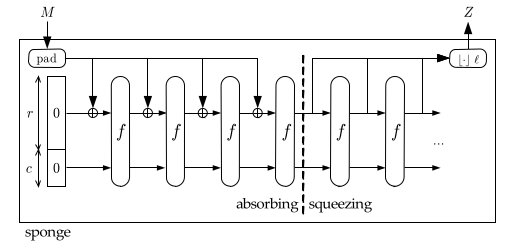
\includegraphics[width=5.5in]{keccakspongeconstruction.jpg}
    \end{center}
    \caption{Sponge construction $Z = Sponge[f, pad, r](M, l)$}
    \label{fig:lab}
  \end{figure}

  The sponge construction is used to build function $SPONGE[f, pad, r]$ which inputs and outputs variable length strings 
  \cite{00016}. It uses fixed length permutation $f$, a padding "pad", and parameter bit rate 'r'. The permutations are 
  operated on fixed number of bits, width $b$. The value $c = b - r$ is the capacity of the sponge function. The width 
  $b$ in Keccak defines the state size which can be any of the following \{25, 50, 100, 200, 400, 800, 1600\} number of 
  bits. 
  
  \begin{figure}
    \begin{center}
      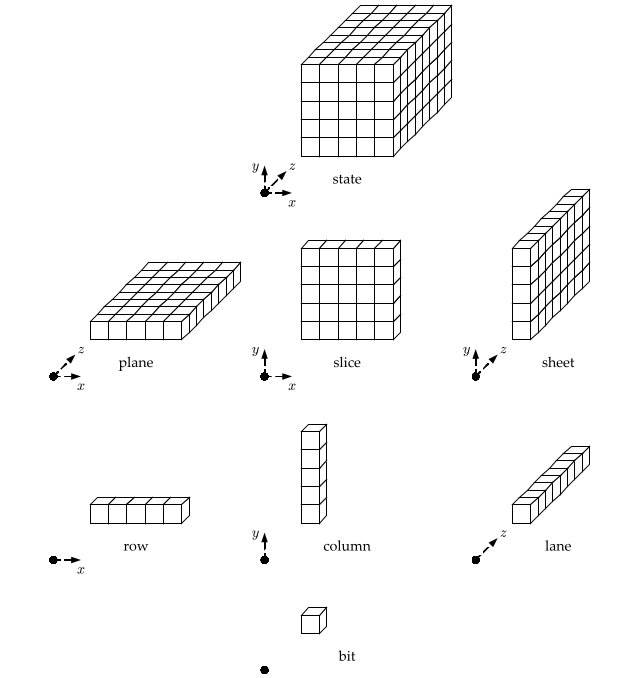
\includegraphics[width=6.5in]{keccakstateterminology.jpg}
    \end{center}
    \caption{Sponge construction $Z = Sponge[f, pad, r](M, l)$}
    \label{fig:lab}
  \end{figure}

  The state in Keccak can be represented as a cube having bits, as shown in figure 3.9. The initial state to the sponge
  construction has value 'b' number of 0 bits(represented as $0^{b}$), and called the root state. The root state has fixed
  value and should not be considered as initial value to sponge construction. The different number of state produces
  the Keccak family of hash function variations denoted by $KECCAK-f[b]$.
  
  The varying number of states can be visualized as state having varying number or $l$ number of slices. The width $b$ is
  defined as $b = 25 \times 2^{l}$, where $l$ takes values from 0 to 6.
  
  \begin{algorithm}
    \caption{The sponge construction $SPONGE[f, pad, r]$}
    \begin{algorithmic}[1]
      \Require $r < b$
      \State {\bf Interface:} Z = sponge($M, l$) with $M \in \mathbb{Z}^{*}_{2}$, integer $ l > 0$ and $Z \in \mathbb{Z}^{l}_{2}$
      \State $P = M \parallel pad[r](\mid M \mid)$
      \State $s = 0^{b}$
      \State \For {$i = 0 \thickspace to \mid P \mid_{r} - 1$}
        \State $s = s \oplus ( P_{i} \parallel 0^{b - r})$
        \State $s = f(s)$
      \State \EndFor
      \State $ Z = \lfloor s \rfloor_{r}$
      \State \While $\mid Z \mid_{r} r < l $
        \State $s = f(s)$
        \State $Z = Z \parallel \lfloor s \rfloor_{r}$
      \State \EndWhile
      \State \Return $\lfloor Z \rfloor_{l}$ 
    \end{algorithmic}
  \end{algorithm}

  Algorithm 3.2 shows how the sponge construction applied to $KECCAK-f[r + c]$, with multi-rate padding. In algorithm 3.2
  length of a string $M$ is denoted by $\mid M \mid $. The string $M$ can also be considered as having blocks of size say x,
  and those number of blocks are shown as $\mid M \mid_{x}$. The $\lfloor M \rfloor_{l}$ denotes the string $M$ truncated to its first $l$ bits.
  
  The multi-rate padding in Keccak is denoted as $pad \thickspace 1 0^{*}1$ , where a bit '1' is appended to message, followed 
  by minimum number of zeros. And lastly a single bit 1, so that resultant block is multiple of block length $b$. Thus 
  Keccak in terms of sponge function can be defined as 

  $KECCAK[r, c] \doteq SPONGE[KECCAK-f[r + c], pad1 0^{*}1, r]$ \\
  Where $ r > 0$ and $r + c$ is the width. The default value of $r$ is $1600 - c$, and the default value of $c$ is 576. \\
  $KECCAK[c] \doteq KECCAK[r = 1600 - c, c], \\
  KECCAK[] \doteq KECCAK[c = 576]$
    
  \subsection{Permutations}

  The $KECCAK-f[b]$ permutations are operated on state represented as a[5][5][w], with w = $2^{l}$, where l can be any value
  from 0 to 6. The position in this 3 dimensional state is given by $a[x][y][z]$ where $x, y \in \mathbb{Z}_{5}$ and $z \in 
  \mathbb{Z}_{w}$. The mapping of the bits from the input message 's' to state 'a' is like this $s[w (5y + x) + z] = a[x][y][z]$.
  The $x, y$ coordinates are taken modulo 5, while the $z$ coordinate is taken as modulo $w$.  \cite{00015}

  There are five steps, for a permutation round R. $R = \zeta \circ \chi \circ \pi \circ \rho \circ \theta$. The permutations are repeated for
  $12 + 2l$ times, with $l$ dependent on the variant chosen. \\
  $
  \theta: a[x][y][z] \gets a[x][y][z] + \displaystyle\sum\limits_{y' = 0}^{4} a[x - 1][y'][z] + \displaystyle\sum\limits_{y' = 0}^{4} a[x + 1][y'][z - 1], \\
  \rho: a[x][y][z] \gets a[x][y][z - (t + 1)(t + 2) / 2], \\
  t \thickspace satisfying \thickspace 0 \leq t < 24 \thickspace and \thickspace
  \begin{pmatrix} 0 & 1 \\ 2 & 3 \end{pmatrix}^{t} \begin{pmatrix} 1 \\ 0 \end{pmatrix} = \begin{pmatrix} x \\ y \end{pmatrix}
  in \thickspace GF(5)^{2 \times 2}, \\
  or \thickspace t = -1 \thickspace if \thickspace x = y = 0, \\
  \pi: a[x][y] \gets a[x'][y'], \thickspace with \thickspace
  \begin{pmatrix} x \\ y \end{pmatrix} = \begin{pmatrix} 0 & 1 \\ 2 & 3 \end{pmatrix} \begin{pmatrix} x' \\ y'\end{pmatrix}, \\
  \chi: a[x] \gets a[x] + (a[x + 1] + 1) a[x + 2], \\
  \zeta: a \gets a + RC[i_{r}].
  $

  The addition and the multiplications are in Galois field GF(2), except for the round constants $RC[i_{r}]$. The round constants 
  are given by

  $RC[i_{r}][0][0][2^{j} - 1] = rc[j + 7i_{r}]$ for all $ 0 \leq j \leq l$, \\
  and the rest are zeros. The value of $rc[t] \in GF(2)$ is output of linear feedback shift register given as 

  $rc[t] = (x^{t} \thickspace mod \thickspace x^{8} + x^{6} + x^{5} + x^{4} + 1)$ mod x in GF(2)[$x$].

  \begin{figure}
    \begin{center}
      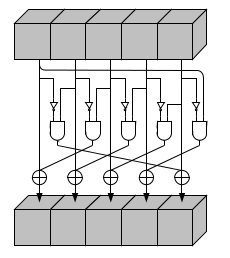
\includegraphics[width=2.3in]{keccakchi.jpg}
    \end{center}
    \caption{$\chi$ applied to a single row.}
    \label{fig:lab}
  \end{figure}

  \begin{algorithm}
    \caption{ $\chi$ transformation KECCAK}
    \begin{algorithmic}[1]
      \State \For {$y = 0 \thickspace to \thickspace 4$}
      \State \For {$x = 0 \thickspace to \thickspace 4$}
      $A[x, y] = a[x, y] \oplus ((NOT \thickspace a[x + 1, y]) \thickspace AND \thickspace a[x + 2, y])$
      \State \EndFor
      \State \EndFor
    \end{algorithmic}
  \end{algorithm}
  
  \begin{figure}
    \begin{center}
      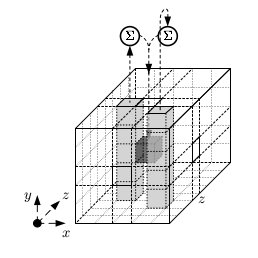
\includegraphics[width=2.7in]{keccaktheta.jpg}
    \end{center}
    \caption{$\theta$ applied to a single bit}
    \label{fig:lab}
  \end{figure}

  \begin{algorithm}
    \caption{ $\theta$ transformation KECCAK}
    \begin{algorithmic}[1]
      \State \For {$x = 0 \thickspace to \thickspace 4$}
      \State $C[x] = a[x, 0]$
      \State \For {$y = 1 \thickspace to \thickspace 4$}
      $C[x] = C[x] \oplus a[x, y]$
      \State \EndFor
      \State \EndFor
      \State \For {$x = 0 \thickspace to \thickspace 4$}
      \State $D[x] = C[x - 1] \oplus ROT(C[x + 1], 1)$
      \State \For {$y = 0 \thickspace to \thickspace 4$}
      \State $A[x, y] = a[x, y] \oplus D[x]$
      \State \EndFor
      \State \EndFor
    \end{algorithmic}
  \end{algorithm}

  \begin{algorithm}
    \caption{ $\pi$ transformation KECCAK}
    \begin{algorithmic}[1]
      \State \For {$x = 0 \thickspace to \thickspace 4$}
      \State \For {$y = 1 \thickspace to \thickspace 4$}
      \State $\begin{pmatrix} X \\ Y \end{pmatrix} = \begin{pmatrix} 0 & 1 \\ 2 & 3 \end{pmatrix} \begin{pmatrix}x \\ y \end{pmatrix}$
      \State $A[X, Y] = a[x, y]$
      \State \EndFor
      \State \EndFor
    \end{algorithmic}
  \end{algorithm}

  \begin{figure}
    \begin{center}
      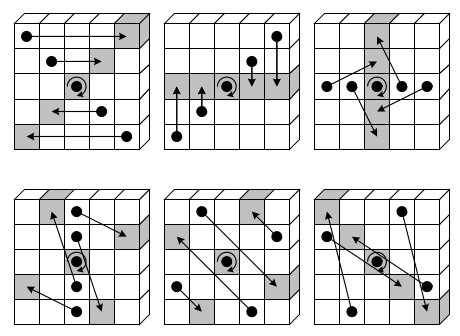
\includegraphics[width=4.75in]{keccakpi.jpg}
    \end{center}
    \caption{$\pi$ applied to a single slice}
    \label{fig:lab}
  \end{figure}

  \begin{algorithm}
    \caption{ $\rho$ transformation KECCAK}
    \begin{algorithmic}[1]
      \State $A[0, 0] = a[0, 0]$
      \State $\begin{pmatrix} x \\ y \end{pmatrix} = \begin{pmatrix} 1 \\ 0 \end{pmatrix}$
      \State \For{$t = 0 \thickspace to \thickspace 23$}
      \State $A[x, y] = ROT(a[x, y], (t + 1)(t + 2) / 2)$
      \State $\begin{pmatrix} x \\ y \end{pmatrix} = \begin{pmatrix} 0 & 1 \\ 2 & 3 \end{pmatrix} \begin{pmatrix}x \\ y \end{pmatrix}$
      \State \EndFor
    \end{algorithmic}
  \end{algorithm}

  \begin{figure}
    \begin{center}
      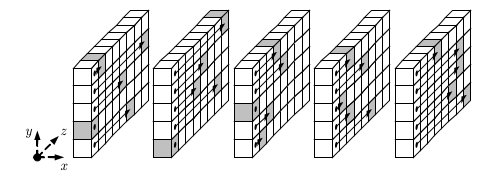
\includegraphics[width=5.1in]{keccakrho.jpg}
    \end{center}
    \caption{$\rho$ transformation applied to lanes}
    \label{fig:lab}
  \end{figure}

  \begin{table}
    \begin{center}
      \begin{tabular}{ c | *{5}{c}}
                & $x = 2$ & $x = 4$ & $x = 0$ & $x = 1$ & $x = 2$ \\ \hline
        $y = 2$ & 153     & 231     & 3       & 10      & 171     \\
        $y = 1$ & 55      & 276     & 36      & 300     & 6       \\
        $y = 0$ & 28      & 91      & 0       & 1       & 190     \\
        $y = 4$ & 120     & 78      & 210     & 66      & 253     \\
        $y = 3$ & 21      & 136     & 105     & 45      & 15      \\
      \end{tabular}
      \caption{Offsets for $\rho$ transformation}
    \end{center}
  \end{table}

